\subsection{WLAN} \label{grund-wlan-subsubsec}

\todo[inline]{Verantwortlich: Kevin, Jonas}

Wireless Local Area Network (WLAN, zu deutsch drahtloses lokales Netzwerk) bezeichnet ein lokales Funknetz nach dem Standard IEEE-802.11, teilweise wird auch synonym (und fälschlicherweise) der Begriff Wi-Fi verwendet. Im Vergleich zu WPAN ist bei WLAN neben einer größere Reichweite und Sendeleistung auch eine höhere Datenübertragungsrate möglich(siehe dazu auch Kapitel 2.3 Bluetooth). Beide Funkstandards arbeiten unter anderem im Frequenzband 2,4GHz (wobei für WLAN  auch höhere Frequenzbänder zur Verfügung stehen z.b. 5 GHz). Der Vorteile von Bluetooth hingegen sind zum einen geringere Hardwarekosten und zum anderen ein geringerer Energiebedarf, was in Batteriebetriebenen Systemen von Vorteil ist.

UDP:
Steht für User Datagram Protocol  und ermöglicht Anwendungen den Versand von Datagrammen in IP basierten Rechnernetzen. UDP gehört zur Transportschicht der Internetprotokollfamilie und ist minimales, verbindungsloses Netzwerkprotokoll. UDP verwendet Ports, um versendete Daten dem richtigen Programm auf dem Zielrechner zukommen zu lassen.  Zu diesem Zweck ist in jedem Datagramm die Portnummer des Dienstes enthalten. Zudem ist mit UDP die Möglichkeit gegeben, eine Prüfsumme mit zu versenden. Mit Hilfe dieser Prüfsumme können fehlerhafte Übertragungen erkannt und gelöscht werden.

\begin{figure}[H] \centering
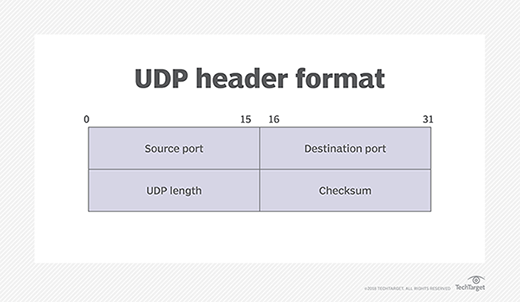
\includegraphics[width=\textwidth]{Images/networking-udp_mobile.png} 
\vspace{-0.3cm} 
\caption{Format eines UDP-Datagramm Headers.}
\label{fig-elise} 
\end{figure}
Hierbei gibt Sourceport die Port-Nummer des sendenden Prozesses an, dies wird benötigt, falls der Empfänger auf das Paket antworten soll. Ist dies nicht der Fall kann dieser Wert aber auch Problemlos auf 0 gesetzt werden. Der Destination port gibt den Prozess an, der das Paket empfangen soll. UDP lenght gibt die Länge des jeweiligen Datagramms, also die Länge von Header + Daten, an. Checksum ist die (optionale) Prüfsumme, dieser Wert wird wenn nicht verwendet auf 0 gesetzt. Gefolgt wird der Header dann von den eigentlichen Nutzdaten (in engl. auch als Payload bezeichnet). Für die eigentliche Übertragung des UDP-Pakets ist das Internet Protokoll(IP) vorgesehen, wodurch dem Paket noch ein weiter Header vorgesetzt wird,  in welchen sich die von dem Internet Protokoll benötigten Daten befinden [Abbildung 2.4.2]

\begin{figure}[H] \centering
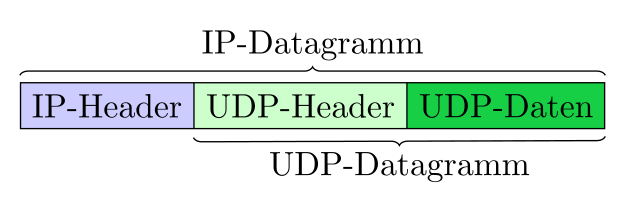
\includegraphics[width=\textwidth]{Images/Udp-package-scheme.png} 
\vspace{-0.3cm} 
\caption{Vollständiges zu übertragendes Paket.}
\label{fig-elise} 
\end{figure}